% Convert with command:
% convert -density 300 pic.pdf -quality 90 pic.png
\documentclass[crop,tikz,border=0pt]{standalone}
\usetikzlibrary{arrows.meta, fit, shapes}
\begin{document}

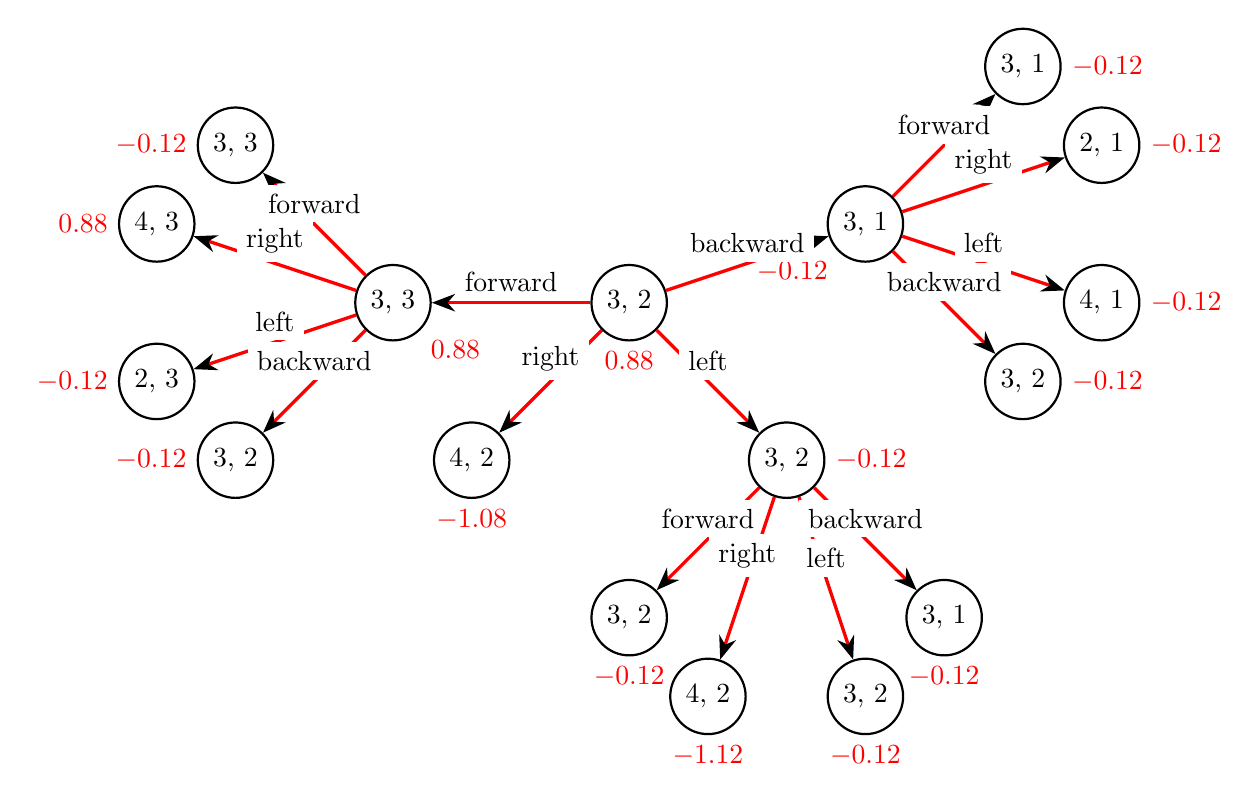
\begin{tikzpicture}
\begin{scope}[
    every node/.style={circle,thick,draw},
    every label/.append style={shape=rectangle,text=red}]
    \node (1) at (0, 0) [shape=circle,draw=black,fill=white,label=below:$0.88$] {3, 2};

    \node (2) at (-3, 0) [shape=circle,draw=black,fill=white,label=south east:$0.88$] {3, 3};

    \node (3) at (-2, -2) [shape=circle,draw=black,fill=white,label=below:$-1.08$] {4, 2};

    \node (4) at (2, -2) [shape=circle,draw=black,fill=white,label=east:$-0.12$] {3, 2};

    \node (5) at (3, 1) [shape=circle,draw=black,fill=white,label=south west:$-0.12$] {3, 1};

    % 2nd node
    \node (6) at (-5, 2) [shape=circle,draw=black,fill=white,label=west:$-0.12$] {3, 3};
    \node (7) at (-6, 1) [shape=circle,draw=black,fill=white,label=west:$0.88$] {4, 3};
    \node (8) at (-6, -1) [shape=circle,draw=black,fill=white,label=west:$-0.12$] {2, 3};
    \node (9) at (-5, -2) [shape=circle,draw=black,fill=white,label=west:$-0.12$] {3, 2};

    % 4th node
    \node (10) at (0, -4) [shape=circle,draw=black,fill=white,label=below:$-0.12$] {3, 2};
    \node (11) at (1, -5) [shape=circle,draw=black,fill=white,label=below:$-1.12$] {4, 2};
    \node (12) at (3, -5) [shape=circle,draw=black,fill=white,label=below:$-0.12$] {3, 2};
    \node (13) at (4, -4) [shape=circle,draw=black,fill=white,label=below:$-0.12$] {3, 1};

    % 5th node
    \node (14) at (5, 3) [shape=circle,draw=black,fill=white,label=east:$-0.12$] {3, 1};
    \node (15) at (6, 2) [shape=circle,draw=black,fill=white,label=east:$-0.12$] {2, 1};
    \node (16) at (6, 0) [shape=circle,draw=black,fill=white,label=east:$-0.12$] {4, 1};
    \node (17) at (5, -1) [shape=circle,draw=black,fill=white,label=east:$-0.12$] {3, 2};
\end{scope}

\begin{scope}[>={Stealth[black]},
              every node/.style={fill=white,rectangle,above},
              every edge/.style={draw=red,very thick}]
    \path [->] (1) edge node {forward} (2);
    \path [->] (1) edge node {right} (3);
    \path [->] (1) edge node {left} (4);
    \path [->] (1) edge node {backward} (5);

    \path [->] (2) edge node {forward} (6);
    \path [->] (2) edge node {right} (7);
    \path [->] (2) edge node {left} (8);
    \path [->] (2) edge node {backward} (9);

    \path [->] (4) edge node {forward} (10);
    \path [->] (4) edge node {right} (11);
    \path [->] (4) edge node {left} (12);
    \path [->] (4) edge node {backward} (13);

    \path [->] (5) edge node {forward} (14);
    \path [->] (5) edge node {right} (15);
    \path [->] (5) edge node {left} (16);
    \path [->] (5) edge node {backward} (17);
\end{scope}
\end{tikzpicture}

% https://texample.net/tikz/examples/scenario-tree/
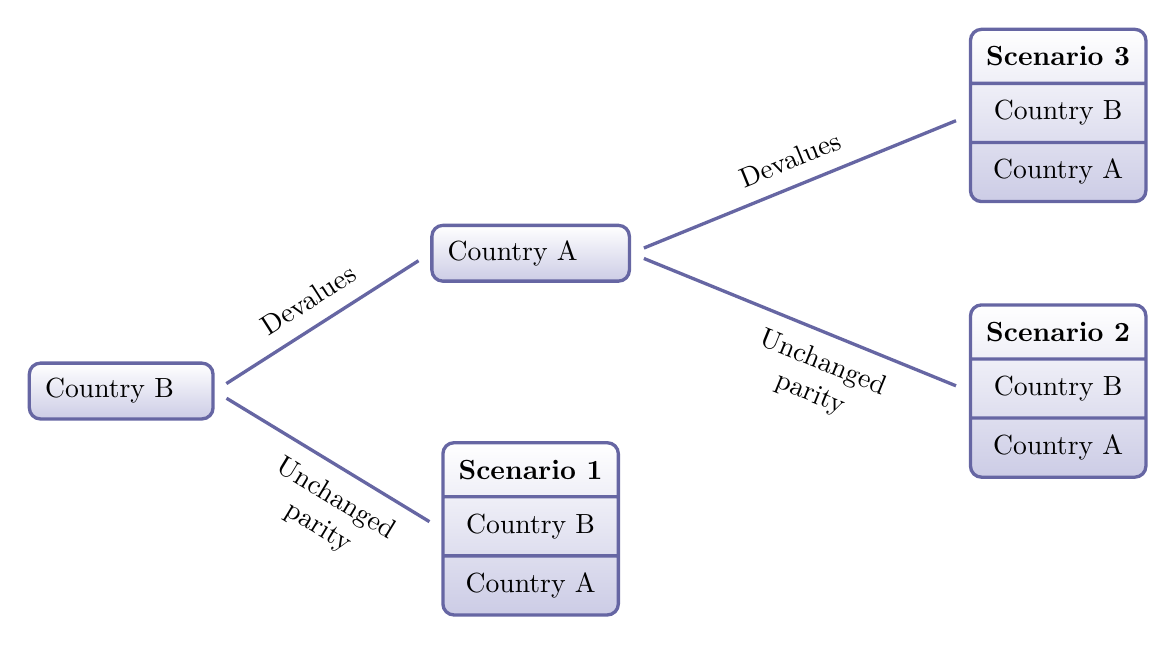
\begin{tikzpicture}[
    grow=right,
    level 1/.style={sibling distance=3.5cm,level distance=5.2cm},
    level 2/.style={sibling distance=3.5cm, level distance=6.7cm},
    edge from parent/.style={very thick,draw=blue!40!black!60,
        shorten >=5pt, shorten <=5pt},
    edge from parent path={(\tikzparentnode.east) -- (\tikzchildnode.west)},
    kant/.style={text width=2cm, text centered, sloped},
    every node/.style={text ragged, inner sep=2mm},
    punkt/.style={rectangle, rounded corners, shade, top color=white,
    bottom color=blue!50!black!20, draw=blue!40!black!60, very
    thick }
    ]

\node[punkt, text width=5.5em] {Country B}
    %Lower part lv1
    child {
        node[punkt] [rectangle split, rectangle split, rectangle split parts=3,
         text ragged] {
            \textbf{Scenario  1}
                  \nodepart{second}
            Country B
                  \nodepart{third}
            Country A
        }
        edge from parent
            node[kant, below, pos=.6] {Unchanged parity}
    }
    %Upper part, lv1
    child {
        node[punkt, text width=6em] {Country A}
        %child 1
        child {
            node [punkt,rectangle split, rectangle split,
            rectangle split parts=3] {
                \textbf{Scenario  2}
                \nodepart{second}
                Country B
                \nodepart{third}
                Country A
            }
            edge from parent
                node[below, kant,  pos=.6] {Unchanged parity}
        }
        %child 2
        child {
            node [punkt, rectangle split, rectangle split parts=3]{
                \textbf{Scenario 3}
                \nodepart{second}
                Country B
                \nodepart{third}
                Country A
            }
            edge from parent
                node[kant, above] {Devalues}}
            edge from parent{
                node[kant, above] {Devalues}}
    };
\end{tikzpicture}

\end{document}
